\section{Numerical Experiments}

To implement and train Triplet Network we used PyTorch 2.0 package \cite{Ansel_2024} designed for performing high-level parallel computations on accelerated hardware. We implemented Stochastic Quantization algorithm using high-level API of a Scikit-learn package \cite{Pedregosa_2011} to ensure compatibility with other components of the package (e.g. model training and evaluation), with an utilization of Numpy package \cite{harris2020array} for parallel tensor computations on CPU. All figures, included in the research, were rendered using Matplotlib package \cite{Hunter_2007}. All source code and experimental results are publicly available on the GitHub repository \cite{Kozyriev_2024}.

The dataset we used for experiments is the original MNIST handwritten digit dataset \cite{lecun2010mnist} (see Fig.~\ref{mnist:fig}) that consists of 60000 gray-scale images of handwritten digits with the resolution of 28x28, each labeled with a class 0-9, with a corresponding set of 10000 test images and their labels. It's important to highlight, that we did not apply data augmentation and preprocessing to both training and test datasets.

\begin{figure}
    \centering
    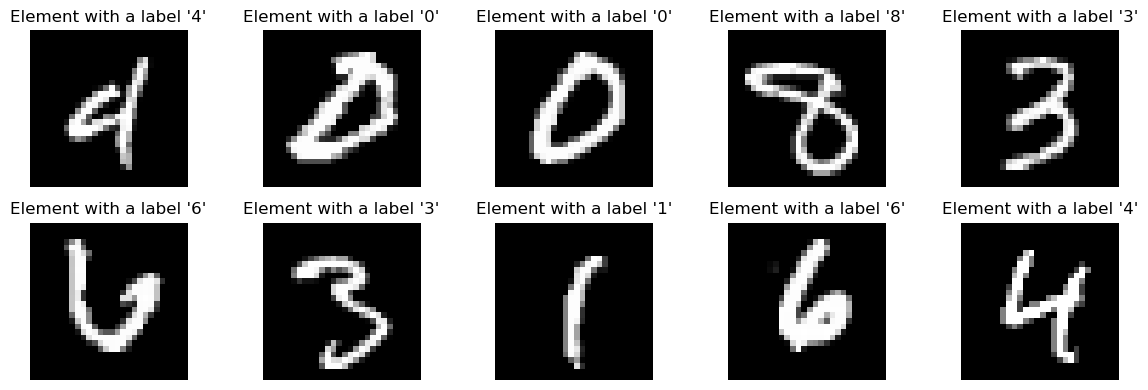
\includegraphics[width=\textwidth]{figures/dataset.png}
    \caption{Training samples from MNIST dataset \cite{lecun2010mnist} with their corresponding labels.} \label{mnist:fig}
\end{figure}

We performed training of image classification models as a semi-supervised problem on different fractions of labeled training data (10\%, 30\%, 60\%, 80\%, 100\%). We split the training dataset with uniform sampling into labeled fraction with given percentage and removed labels from remained training data. For Triplet Network we used Convolutional Network, consisting of 2 Convolutional Layers with 3x3 Convolutional Filters (having feature map dimensions as 32 and 64 respectively with $\text{stride}=1$ and $\text{padding}=1$) and 2x2 Max-Pooling Filters, following 2 Dense Layers. Each layer as an activation function uses ReLU. We trained separate models of Triplet Network on each labeled fraction with following hyperparameters: 50 epochs, $1000 \times fraction$ samples in batch size, learning rate $ \rho = 10^{-3} $, and $ l_2 $ regularization rate $ \lambda = 10^{-5} $. For triplet loss (\ref{triplet-loss-func:eq}) and triplet mining (\ref{semi-hard-triplet-mining:eq}) we selected margin hyperparameter as $\alpha = 1.0$. To let Triplet Network capture meaningful features into latent space, while being able to visualize results, we chose a dimensionality of the latent space as $\mathbb{R}^3$ (see Fig.~\ref{latent-space:fig}).

\begin{figure}
    \centering
    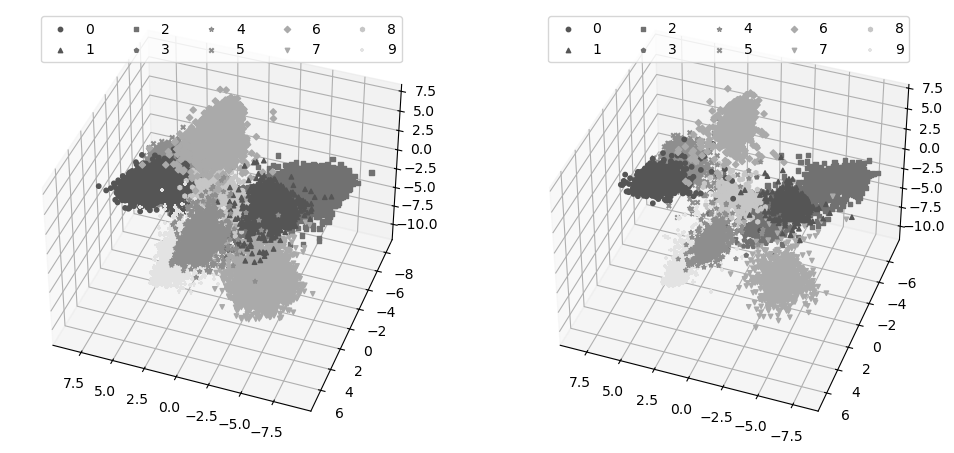
\includegraphics[width=\textwidth]{figures/latent_space.png}
    \caption{Latent representations of images in train dataset (left) and test dataset (right) projected by Triplet Network with each element marked according to the label (0-9). We can assume the Triplet  successfully captured the features during the training phase, given its ability to group elements with same label into a cluster.} \label{latent-space:fig}
\end{figure}

We used Triplet Network to project latent representations on $\mathbb{R}^3$ space from training data (both labeled and unlabeled fractions), which we then employed to train Stochastic Quantization algorithm as an unsupervised learning model. For each latent representations on different labeled data fraction, we trained a Stochastic Quantization, and its adaptive variants (\ref{momentum-update-rule:eq})-(\ref{adam-update-rule:eq}). We employed same initialization strategy for each variant, which is KMeans++ (\ref{kmeans-plus-plus-init:eq}), and same rank hyperparameter $ r = 3 $. However, the learning rate of each variant was different for ensuring the convergence: for SGD, Momentum and NAG we chose $ \rho = 0.001 $, for AdaGrad $ \rho = 0.9 $, and for RMSProp and ADAM $ \rho = 0.01 $. With this choice of hyperparameters, all of Stochastic Quantization variants converged to the global optima (see Fig.~\ref{quants:fig}), while most of them converged on the first iteration (see Fig.~\ref{convergence:fig}).

\begin{figure}
    \centering
    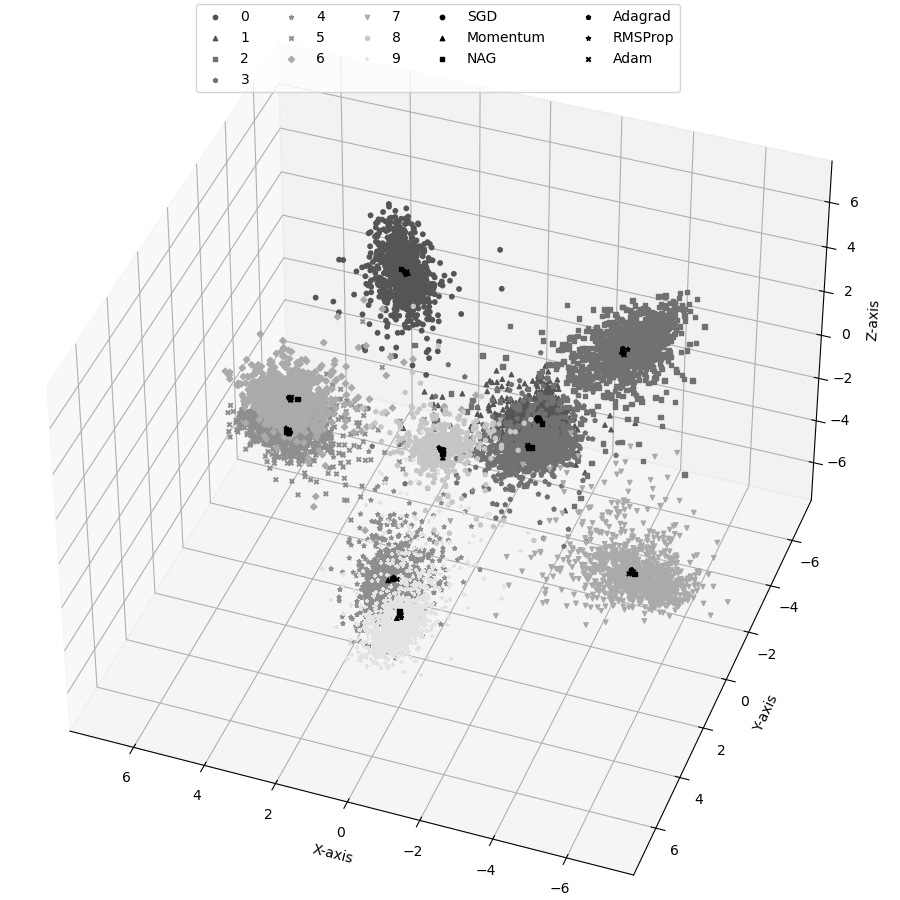
\includegraphics[width=0.9\textwidth]{figures/sq_quants.png}
    \caption{Optimal positions of quants for each Stochastic Quantization variant (labeled with the name of the variant) on the latent space relative to labeled elements (0-9) from test dataset.} \label{quants:fig}
\end{figure}

\begin{figure}
    \centering
    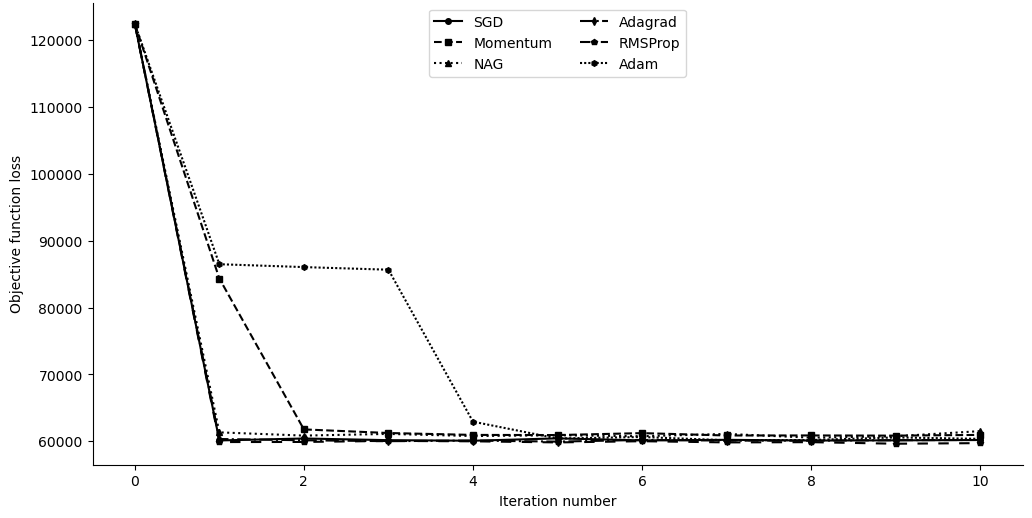
\includegraphics[width=\textwidth]{figures/sq_convergence_full_dataset.png}
    \caption{Convergence speed comparison of Stochastic Quantization variants on latent representations of trained data with 100\% labeled fraction.} \label{convergence:fig}
\end{figure}

The accuracy of trained classification models, being a combination of Triplet Network and Stochastic Quantization, were compared using the F1-score metric \cite{Chinchor_1992} for weighted multi-label classification. Our experiments showed that our approach managed to get results comparable to state-of-the-art results with Triplet Network and Siamese Network provided in \cite{Hoffer_2015}, even with limited amount of labeled data:

\begin{table} 
\caption{Classification accuracy comparison on MNIST dataset \cite{lecun2010mnist}}
\label{accuracy:table}
    \begin{tabularx}{\textwidth}{|X|*{5}{c|}}
        \hline
        \multirow{2}{*}{Algorithm} & \multicolumn{5}{c|}{Percentage of Training Data} \\
        \cline{2-6}
        & 10\% & 30\% & 60\% & 80\% & 100\% \\
        \hline
        Triplet Network + KNN         & - & - & - & - & 99.54\% \\
        Siamese Network + KNN         & - & - & - & - & 97.90\% \\
        Triplet Network + SQ-SGD      & 94.67\% & 98.14\% & 98.23\% & 98.17\% & 98.26\% \\
        Triplet Network + SQ-Momentum & 92.97\% & 98.20\% & 98.26\% & 98.14\% & 98.24\% \\
        Triplet Network + SQ-NAG      & 94.12\% & 98.15\% & 98.29\% & 98.16\% & 98.25\% \\
        Triplet Network + SQ-AdaGrad  & 94.59\% & 98.11\% & 98.24\% & 98.18\% & 98.30\% \\
        Triplet Network + SQ-RMSProp  & 94.34\% & 98.16\% & 98.19\% & 98.17\% & 98.27\% \\
        Triplet Network + SQ-ADAM     & 93.01\% & 98.18\% & 98.23\% & 98.18\% & 98.25\% \\
        \hline
    \end{tabularx}
\end{table}
